\clearpage
\phantomsection
\setcounter{secnumdepth}{3}

\setcounter{chapter}{3}
\chapter[{KẾT QUẢ THỰC NGHIỆM VÀ ĐÁNH GIÁ}]{Kết quả thực nghiệm và đánh giá}

Chương này phân tích kết quả thực nghiệm theo bốn nhóm gắn với mục tiêu đề tài: kỹ thuật khám phá, CL, vùng bão hòa entropy và nút thắt quan sát. Các nhóm này được sắp xếp theo mạch từ so sánh tác động của từng kỹ thuật huấn luyện đến phân tích các giới hạn còn lại của tác nhân. Mục~\ref{sec:eval_metrics} định nghĩa độ đo và tiêu chí đánh giá trước khi dùng; các mục sau phân tích kết quả theo từng nhóm.

\textbf{Lộ trình phân tích kết quả.} Để người đọc theo dõi mạch phân tích, Bảng~\ref{tab:results_storyline} ánh xạ từng nhóm câu hỏi nghiên cứu (Q1--Q3) và mục tiêu (MT1--MT4) với các mục của chương này. Trong đó, Q1 tập trung vào hiệu quả của từng kỹ thuật, Q2 xem xét tác động khi kết hợp với CL, còn Q3 đi vào vai trò của biểu diễn quan sát và tín hiệu điều hướng.

\begin{table}[H]
    \centering
    \small
    \caption{Tổng quan câu hỏi nghiên cứu, mục tiêu và cấu hình phân tích}
    \label{tab:results_storyline}
    \begin{tabular}{|p{4cm}|p{4cm}|p{5cm}|}
        \hline
        \textbf{Câu hỏi / MT} & \textbf{Mục trả lời} & \textbf{Run chính được phân tích} \\
        \hline
        Q1 (kỹ thuật khám phá ICM/RND) & Mục~\ref{sec:exploration_techniques} & run34 vs run35, run36 \\
        \hline
        Q1 (bộ nhớ LSTM) & Mục~\ref{sec:lstm_results} & run34 vs run42 \\
        \hline
        Q1 (CL) & Mục~\ref{sec:curriculum_results} & run34 vs run46 \\
        \hline
        Q2 (kết hợp CL + LSTM/ICM) & Mục~\ref{sec:curriculum_combinations} & run46 vs run47, run50 \\
        \hline
        MT1 + MT2 (môi trường) & Mục~\ref{sec:spawn_strategy_results}, Mục~\ref{sec:reward_v2_results} & run54, run55 \\
        \hline
        MT3 (vùng bão hòa entropy) & Mục~\ref{sec:entropy_plateau_results} & toàn bộ 207D + run62 \\
        \hline
        Q3 + MT4 (nút thắt quan sát) & Mục~\ref{sec:run59_path_informed}, Mục~\ref{sec:run62_local_grid} & run59, run62 \\
        \hline
    \end{tabular}
\end{table}

\section{Độ đo và tiêu chí đánh giá}
\label{sec:eval_metrics}

Tất cả chỉ số được trích từ log TensorBoard. Dưới đây là định nghĩa các độ đo chính và tiêu chí được sử dụng trong phần phân tích:

\begin{itemize}
    \item \textbf{cumulative\_reward}: tổng phần thưởng tích lũy mỗi lượt chơi theo thang thưởng đang dùng. Run55 dùng v2 nên không so sánh trực tiếp với v1.
    \item \textbf{clear\_rate}: tỷ lệ lượt chơi tác nhân tiêu diệt toàn bộ kẻ địch. Tiêu chí thành công: clear\_rate $\geq 0.5$.
    \item \textbf{kills/episode}: số kẻ địch trung bình bị tiêu diệt mỗi lượt chơi.
    \item \textbf{entropy (nat)}: độ hỗn loạn của phân phối hành động. Mốc cực đại lý thuyết là $\ln(3)+\ln(3)+\ln(3)+\ln(9) \approx 5.49$ nat; vùng bão hòa quan sát được quanh 4.40 nat.
    \item \textbf{tail-50}: trung bình 50 lượt chơi cuối, dùng cho các so sánh chính trừ khi có ghi chú khác.
    \item \textbf{rolling\_reward\_200k}: phần thưởng trung bình động theo từng khoảng 200k bước, dùng để vẽ xu hướng học.
    \item \textbf{reward\_hard\_from\_140k}: phần thưởng trung bình sau khi CL chuyển vào mức Khó (từ bước $\sim$140k).
    \item \textbf{damage\_dealt} (\textit{Dmg+}) và \textbf{damage\_taken} (\textit{Dmg-}): tổng sát thương gây ra và nhận vào mỗi lượt chơi.
    \item \textbf{useful\_dash\_rate} (\textit{Lướt+}): tỷ lệ lần lướt hữu ích trên tổng số lần lướt.
    \item \textbf{dash\_per\_decision} (\textit{Lướt/dec}): tần suất chọn hành động lướt trên tổng số bước quyết định.
    \item \textbf{policy\_loss} (\textit{P-loss}) và \textbf{value\_loss} (\textit{V-loss}): hai giá trị loss của PPO, dùng để nhận diện bất ổn chính sách hoặc Critic chưa theo kịp.
    \item \textbf{value\_estimate} (\textit{V-est}): ước lượng giá trị trung bình của Critic.
    \item \textbf{inverse\_loss} (\textit{ICM inv.}): cross-entropy của mô hình ngược trong ICM dự đoán hành động từ hai trạng thái liên tiếp. Mốc 5.49 nat chỉ dùng làm tham chiếu.
    \item \textbf{intrinsic\_reward} (\textit{Int. rew.}): phần thưởng nội tại trung bình của ICM/RND.
\end{itemize}

\textit{Hạn chế so sánh}: run34--run42 dừng ở 1.0M bước; run46+ chạy đến 3.0M bước. So sánh liên nhóm là so sánh giữa cấu hình hoàn chỉnh, không phải tại cùng số bước.

\phantomsection\label{sec:eval_thresholds}
\textbf{Quy ước đánh giá thực nghiệm.}

Các mục tiêu MT1--MT4 đã được xác định ở phần Mở đầu. Trong chương này, các mục tiêu đó được đối chiếu bằng một số quy ước định lượng để việc diễn giải kết quả nhất quán và hạn chế phụ thuộc vào nhận định chủ quan:

\begin{itemize}
    \item \textbf{Đạt MT1}. Cấu hình được xem là đạt mục tiêu chiến đấu hiệu quả khi tỷ lệ dọn phòng tail-50 trên nhóm bản đồ Khó đạt ít nhất $0.5$.
    \item \textbf{Cải thiện đáng kể}. So với cấu hình cơ sở, phần thưởng hoặc tỷ lệ dọn phòng cần tăng trên $20\%$. Mức tăng từ $10\%$ đến $20\%$ được xem là cải thiện nhẹ; dưới $10\%$ được xem là tương đương nếu cùng thang thưởng.
    \item \textbf{Vượt vùng bão hòa entropy}. Entropy tail-50 cần giảm hơn $1$ nat so với mức $4.40$ nat quan sát được trong nhóm thí nghiệm cô lập biến 207D ở 1--3M bước.
    \item \textbf{ICM học biểu diễn hữu ích}. Mất mát của mô hình ngược cần giảm rõ so với entropy ngẫu nhiên lý thuyết $5.49$ nat và thấp hơn đáng kể vùng entropy chính sách quan sát được quanh $4.40$ nat. Nếu mất mát của mô hình ngược vẫn quanh hoặc trên $4.0$ nat, biểu diễn được xem là có học một phần nhưng chưa đủ mạnh để giải thích cải thiện hành vi.
\end{itemize}

Các ngưỡng này không phải mục tiêu mới của đề tài, mà là thước đo thực nghiệm dùng để đọc các kết quả trong Chương~4 và tổng kết lại ở Chương~5. Đặc biệt, ngưỡng clear\_rate $0.5$ chỉ xác định mức dọn phòng ổn định trên tập bản đồ thực nghiệm hiện tại; nó chưa thay thế cho đánh giá khái quát hóa trên tập bản đồ giữ riêng.

\begin{table}[H]
    \centering
    \scriptsize
    \setlength{\tabcolsep}{4pt}
    \renewcommand{\arraystretch}{1.15}
    \caption{Các chỉ số hành vi chính ở cuối quá trình huấn luyện}
    \label{tab:run_metrics_main}
    \begin{tabular}{l p{3.0cm} c c c c c c c c}
        \toprule
        \textbf{Run} & \textbf{Thiết lập} & \textbf{Bước} & \textbf{Reward} & \textbf{Clear} & \textbf{Kills} & \textbf{Dmg+} & \textbf{Dmg-} & \textbf{Lướt+} & \textbf{Ent} \\
        \midrule
        run34 & PPO cơ sở & 1.00M & 2.073 & 0.129 & 0.721 & 25.977 & 16.867 & 0.149 & 4.408 \\
        run35 & PPO + ICM & 1.00M & 2.416 & 0.173 & 0.752 & 26.614 & 15.242 & 0.116 & 4.407 \\
        run36 & PPO + RND & 1.00M & 2.487 & 0.159 & 0.796 & 28.068 & 14.013 & 0.107 & 4.406 \\
        run42 & PPO + LSTM & 1.00M & 2.411 & 0.163 & 0.769 & 27.140 & 15.775 & 0.132 & 4.405 \\
        run46 & PPO + CL & 3.00M & 3.843 & 0.267 & 0.994 & 35.135 & 19.368 & 0.245 & 4.409 \\
        run47 & CL + LSTM & 3.00M & 3.765 & 0.241 & 0.921 & 32.884 & 16.420 & 0.228 & 4.405 \\
        run50 & CL + ICM & 3.00M & 4.369 & 0.273 & 1.016 & 36.161 & 23.132 & 0.334 & 4.411 \\
        run54 & 4 bậc, cố định--ngẫu nhiên & 3.00M & 3.925 & 0.242 & 0.945 & 33.673 & 17.966 & 0.179 & 4.407 \\
        run55 & CL + hàm thưởng v2 & 3.00M & 9.337 & 0.267 & 1.014 & 35.685 & 21.312 & 0.240 & 4.407 \\
        run62 & Lưới cục bộ + aggressive\_seek + ICM + 4 bậc & 40.82M & 14.913 & 0.666 & 1.582 & 49.193 & 23.314 & 0.439 & 3.048 \\
        \bottomrule
    \end{tabular}
    \vspace{10pt}
    
    \begin{minipage}{0.96\textwidth}
        \small\textit{Ghi chú}: run62 không so sánh trực tiếp với các lần chạy khác do khác biệt về kích thước quan sát (432 chiều so với 207), số bước huấn luyện (40.82M so với 1--3M bước), siêu tham số PPO điều chỉnh và các thay đổi môi trường bổ sung. Run62 được đưa vào bảng như cấu hình tham chiếu mở rộng, không dùng như một so sánh trực tiếp.
    \end{minipage}
\end{table}

\begin{table}[H]
    \centering
    \scriptsize
    \setlength{\tabcolsep}{5pt}
    \renewcommand{\arraystretch}{1.15}
    \caption{Các chỉ số loss, chính sách và phần thưởng nội tại}
    \label{tab:run_metrics_aux}
    \begin{tabular}{l p{3.5cm} c c c c c c}
        \toprule
        \textbf{Run} & \textbf{Thiết lập} & \textbf{P-loss} & \textbf{V-loss} & \textbf{V-est} & \textbf{Lướt/dec} & \textbf{ICM inv.} & \textbf{Int. rew.} \\
        \midrule
        run34 & PPO cơ sở & 0.016 & 0.140 & 0.170 & 0.0002 & -- & -- \\
        run35 & PPO + ICM & 0.017 & 0.072 & 0.169 & 0.0002 & 4.360 & 0.150 \\
        run36 & PPO + RND & 0.016 & 0.071 & 0.167 & 0.0002 & -- & 0.099 \\
        run42 & PPO + LSTM & 0.082 & 0.168 & 0.178 & 0.0002 & -- & -- \\
        run46 & PPO + CL & 0.017 & 0.207 & 0.401 & 0.0005 & -- & -- \\
        run47 & CL + LSTM & 0.079 & 0.229 & 0.380 & 0.0004 & -- & -- \\
        run50 & CL + ICM & 0.016 & 0.113 & 0.483 & 0.0011 & 4.337 & 0.185 \\
        run54 & 4 bậc, cố định--ngẫu nhiên & 0.017 & 0.200 & 0.416 & 0.0005 & -- & -- \\
        run55 & CL + hàm thưởng v2 & 0.016 & 0.662 & 0.962 & 0.0005 & -- & -- \\
        run62 & Lưới cục bộ + aggressive\_seek + ICM + 4 bậc & 0.017 & 0.231 & 2.615 & -- & 3.032 & 0.008 \\
        \bottomrule
    \end{tabular}
\end{table}

Trong Bảng~\ref{tab:run_metrics_main}, cột Reward là \textbf{reward\_tail50} với các lần chạy không dùng CL và \textbf{reward\_hard\_from\_140k} với các lần chạy dùng CL; các cột Clear, Kills, Dmg+/Dmg-, Lướt+ và Ent lần lượt là \textbf{cleared\_tail50}, \textbf{kills\_tail50}, \textbf{damage\_dealt/taken\_tail50}, \textbf{useful\_dash\_rate\_tail50} và \textbf{entropy\_tail50}. Bảng~\ref{tab:run_metrics_aux} giữ các tín hiệu chẩn đoán quan trọng: mất mát chính sách, mất mát giá trị, ước lượng giá trị ngoại tại, tần suất lướt, mất mát của mô hình ngược trong ICM và phần thưởng nội tại. Các cột trống được ký hiệu ``--'' vì run tương ứng không sử dụng kỹ thuật đó.

\begin{figure}[H]
    \centering
    
\includegraphics[width=0.98\textwidth]{figures/training/training_reward_curves.png}
    \caption{Diễn biến phần thưởng theo số bước huấn luyện của các cấu hình chính}
    \label{fig:training_reward_curves}
\end{figure}

Các lần chạy không dùng CL kết thúc ở 1M bước nên được hiển thị bằng đoạn nằm ngang sau mốc này để thuận tiện so sánh trực quan trên cùng một trục thời gian. Do nhóm không dùng CL chủ yếu dừng ở 1M bước còn nhóm dùng CL chạy đến 3M bước, các so sánh cuối quá trình phản ánh hiệu quả của cấu hình hoàn chỉnh đã thực nghiệm, chưa phải so sánh tuyệt đối tại cùng số bước huấn luyện. Riêng run55 sử dụng hàm thưởng v2, do đó giá trị phần thưởng tuyệt đối của run này không được so sánh trực tiếp với các lần chạy dùng hàm thưởng v1; hình chủ yếu nhằm quan sát xu hướng học và vị trí tương đối giữa các nhóm thí nghiệm.

\section{Kỹ thuật khám phá và bộ nhớ}
\label{sec:exploration_group}

Nhóm thí nghiệm đầu tiên trả lời Q1 bằng cách cô lập từng kỹ thuật bổ sung vào PPO cơ sở: phần thưởng nội tại ICM và RND để thúc đẩy khám phá, và bộ nhớ LSTM để khai thác lịch sử quan sát. Tất cả các lần chạy trong nhóm này đều được huấn luyện đến 1M bước mà không dùng CL.

\subsection{Ảnh hưởng của các kỹ thuật khám phá}
\label{sec:exploration_techniques}

Nhóm thí nghiệm đầu tiên trả lời phần đầu của Q1: liệu phần thưởng nội tại có giúp tác nhân vượt qua giai đoạn khám phá ban đầu hay không. Run34 là cấu hình PPO cơ sở, chưa áp dụng CL. Sau 1 triệu bước huấn luyện, phần thưởng tích lũy trung bình trên 50 lượt chơi cuối đạt 2.073, tỷ lệ dọn phòng trung bình đạt 0.129 và tỷ lệ dọn phòng cao nhất đạt 0.50. Kết quả này cho thấy tác nhân đã học được một số hành vi cơ bản như tiếp cận và tấn công kẻ địch, nhưng chưa duy trì ổn định khả năng dọn phòng trên nhóm bản đồ khó.

Hai biến thể phần thưởng nội tại được đánh giá là ICM ở run35 và RND ở run36. ICM đạt phần thưởng tail-50 là 2.416, RND đạt 2.487. Cả hai đều cải thiện so với PPO cơ sở, nhưng mức tăng còn tương đối nhỏ và chưa tạo ra thay đổi rõ rệt trong hành vi của tác nhân. Có thể thấy khó khăn chính của môi trường không chỉ nằm ở việc thiếu tín hiệu thúc đẩy khám phá, mà còn đến từ độ khó ban đầu của bản đồ và nhiệm vụ chiến đấu.

% \begin{figure}[H]
%     \centering
%     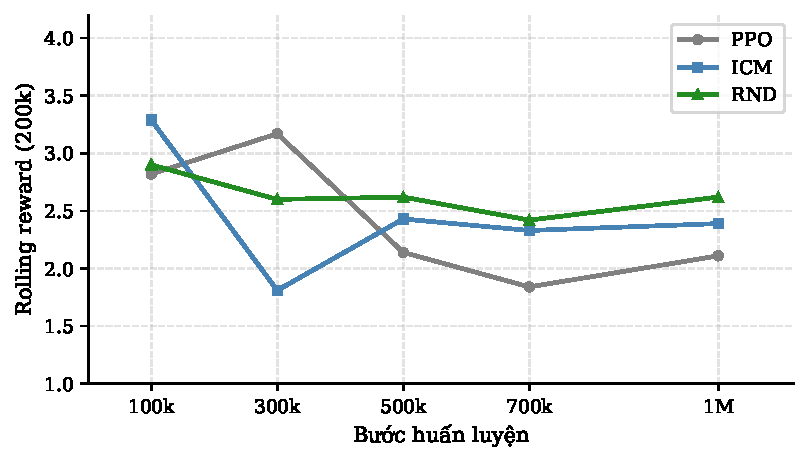
\includegraphics[width=0.85\textwidth]{figures/training/fig42_reward_ppo_icm_rnd.pdf}
%     \caption{Phần thưởng trung bình trượt 200k bước của PPO baseline, ICM và RND trong 1M bước đầu}
%     \label{fig:baseline_intrinsic_reward}
% \end{figure}

\subsubsection{ICM và dấu hiệu biểu diễn chưa ổn định}

ICM học một mô hình ngược dự đoán hành động từ trạng thái trước và sau \cite{Pathak2017}. Với không gian hành động rời rạc nhiều nhánh $(3,3,3,9)$, tổng số tổ hợp hành động là 243, tương ứng entropy ngẫu nhiên lý thuyết khoảng 5.49 nat nếu mọi tổ hợp được chọn đều. Trong run35, mất mát của mô hình ngược dao động quanh 4.36, thấp hơn mức ngẫu nhiên lý thuyết. Điều này cho thấy ICM không hoàn toàn dự đoán ngẫu nhiên, mà đã học được một phần quan hệ giữa thay đổi trạng thái và hành động của tác nhân. Tuy nhiên, giá trị này vẫn gần vùng entropy chính sách khoảng 4.40 nat quan sát ở nhiều lần chạy 207 chiều, nên biểu diễn học được chưa đủ ổn định để tạo cải thiện hành vi rõ rệt.

Khó khăn của ICM đến từ đặc thù môi trường chiến đấu có bản đồ sinh tự động. Cùng một hành động có thể dẫn đến hệ quả rất khác nhau tùy vị trí tường, khoảng cách tới kẻ địch, hướng đạn, thời gian hồi chiêu và cách bố trí bản đồ; ngược lại, hai hành động khác nhau cũng có thể tạo ra thay đổi trạng thái gần giống nhau nếu tác nhân bị kẹt hoặc không nhìn thấy mục tiêu. Vì quan sát 207 chiều chủ yếu mô tả tín hiệu chiến đấu cục bộ và chưa cung cấp đầy đủ cấu trúc đường đi, phần thưởng nội tại có thể khuyến khích khám phá nhưng chưa chắc dẫn tới chuỗi hành vi hữu ích như tiếp cận, căn hướng, né đạn và kết liễu kẻ địch. Điều này giải thích vì sao ICM chạy độc lập chỉ cải thiện hạn chế, còn khi ghép với CL ở run50 mới cho kết quả tốt hơn.

\begin{figure}[H]
    \centering
    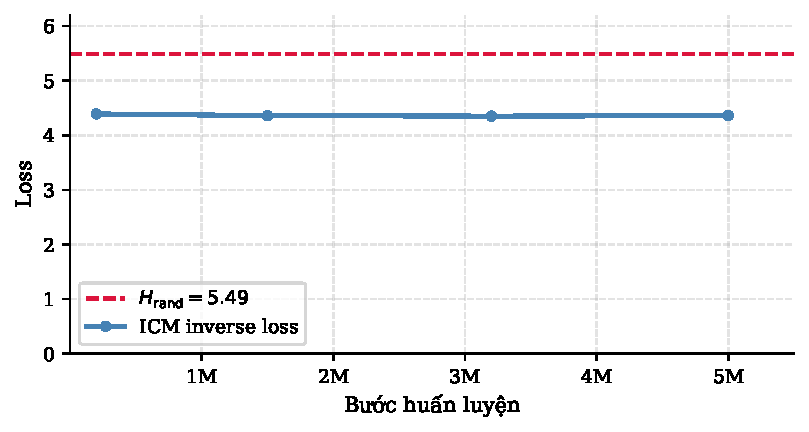
\includegraphics[width=0.85\textwidth]{figures/training/fig43_icm_inverse_loss.pdf}
    \caption{Mất mát của mô hình ngược trong ICM giảm so với mức ngẫu nhiên lý thuyết nhưng vẫn gần vùng entropy chính sách}
    \label{fig:icm_inverse_plateau}
\end{figure}

RND không cần dự đoán hành động nên tránh được hiện tượng mất mát của mô hình ngược suy giảm chất lượng \cite{Burda2018}, nhưng phần thưởng nội tại của run36 giảm nhanh về mức nhỏ khi mô hình dự đoán quen với phân phối quan sát. Vì vậy, RND nhỉnh hơn ICM nhẹ ở phần thưởng tail-50, nhưng vẫn chưa vượt mốc so sánh đáng kể.

\subsection{Vai trò của bộ nhớ LSTM}
\label{sec:lstm_results}

Phần tiếp theo của Q1 kiểm tra liệu bộ nhớ tuần tự có giúp tác nhân xử lý hồi chiêu, đạn và trạng thái khuất tầm nhìn hay không. Run42 thêm LSTM với bộ nhớ kích thước 256 và chuỗi quan sát dài 64 bước. Khác với ICM/RND, LSTM có xu hướng học chậm nhưng tăng dần về cuối. Phần thưởng trung bình trượt 200k bước tăng từ 1.64 ở mốc 100k lên 2.71 ở mốc 1M. Xu hướng này phù hợp với giả thuyết bộ nhớ có ích cho hồi chiêu, đạn và trạng thái khuất tầm nhìn; tuy nhiên lợi ích chưa đủ lớn để tạo cải thiện đáng chú ý trong quy mô huấn luyện hiện tại.

\begin{figure}[H]
    \centering
    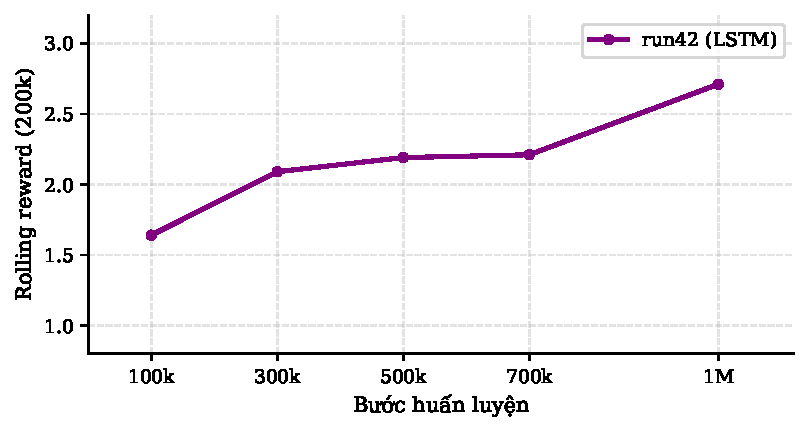
\includegraphics[width=0.85\textwidth]{figures/training/fig44_lstm_trend.pdf}
    \caption{Xu hướng học của run42 khi bổ sung LSTM}
    \label{fig:lstm_trend}
\end{figure}

Như vậy, kiến trúc bộ nhớ có thể là hướng cải tiến phụ, nhưng chưa giải quyết được vấn đề chính của môi trường: tác nhân vẫn phải học từ nhóm Khó quá rộng và khó nhận được chuỗi phần thưởng thành công đủ thường xuyên.

\section{Học theo lộ trình và các biến thể}
\label{sec:curriculum_group}

Nhóm thí nghiệm thứ hai trả lời Q2: sau khi phần thưởng nội tại và bộ nhớ chỉ tạo cải thiện nhẹ, CL được kiểm tra như cơ chế chính giảm độ khó ban đầu của môi trường. Nhóm này bao gồm cấu hình CL cơ sở, kết hợp với LSTM hoặc ICM, biến thể chiến lược vị trí sinh, và thử nghiệm thiết kế lại hàm thưởng.

\subsection{Vai trò của học theo lộ trình}
\label{sec:curriculum_results}

Sau khi ICM, RND và LSTM chỉ tạo cải thiện nhẹ trong nhóm chạy 1M bước, CL được kiểm tra như cơ chế giảm độ khó ban đầu của môi trường. Run46 là cấu hình thể hiện rõ nhất tác động này trong phạm vi các lần chạy đã thực hiện. Thay vì đưa tác nhân vào ngay nhóm bản đồ Khó, CL bắt đầu ở mức Dễ, chuyển sang Trung bình tại khoảng 70k bước và chuyển sang Khó tại khoảng 140k bước. Cách tổ chức này giúp tác nhân có thêm cơ hội học các hành vi cơ bản như tiếp cận kẻ địch, căn hướng tấn công và né tránh trước khi gặp các bố cục khó hơn.

Sau khi vào nhóm Khó, phần thưởng trung bình của run46 đạt 3.843, cao hơn khoảng 85\% so với mốc so sánh tail-50 2.073 của PPO cơ sở. Kết quả này cho thấy CL không chỉ tăng phần thưởng, mà còn làm quá trình học ổn định hơn bằng cách giảm áp lực khám phá ở giai đoạn đầu. Tuy nhiên, do run46 được huấn luyện dài hơn nhóm không dùng CL, mức cải thiện này cần được hiểu như xu hướng thực nghiệm trong các cấu hình đã chạy, chưa phải so sánh tuyệt đối tại cùng số bước huấn luyện.

\begin{figure}[H]
    \centering
    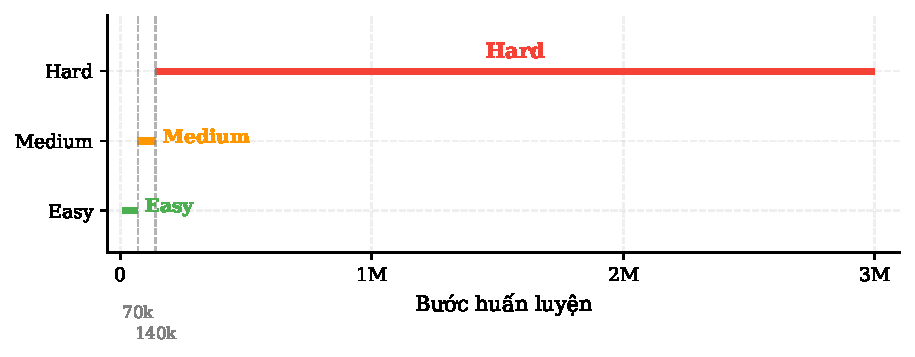
\includegraphics[width=0.85\textwidth]{figures/training/fig45_run46_lesson_transition.pdf}
    \caption{Quá trình chuyển mức độ khó của run46: Dễ $\rightarrow$ Trung bình $\rightarrow$ Khó}
    \label{fig:run46_lesson_transition}
\end{figure}

Phần thưởng theo từng mức độ khó của run46 cho thấy trung bình trên mức Dễ đạt 6.364, trên mức Trung bình đạt 4.181 và trên mức Khó đạt 3.843. Khi vào nhóm Khó, diễn biến phần thưởng không tăng tuyến tính mà dao động trong vùng 3.1--4.2 khi lấy trung bình động trên mỗi khoảng 200k bước. Dao động này là hợp lý vì nhóm Khó có nhiều cấu hình bản đồ hơn, đồng thời vị trí sinh và phân bố kẻ địch cũng đa dạng hơn.

\begin{figure}[H]
    \centering
    
\includegraphics[width=0.98\textwidth]{figures/training/curriculum_reward_trend.png}
    \caption{Xu hướng phần thưởng trong các cấu hình dùng CL}
    \label{fig:curriculum_reward_trend}
    \vspace{0.2em}
    \begin{minipage}{0.94\textwidth}
        \small
        Diễn biến phần thưởng không tăng đều sau khi vào mức Khó mà dao động quanh một vùng ổn định. Run50 cao hơn run46 ở phần sau quá trình huấn luyện -- ICM chỉ phát huy rõ khi chính sách đã có kỹ năng cơ bản từ CL.
    \end{minipage}
\end{figure}

\begin{figure}[H]
    \centering
    
\includegraphics[width=0.98\textwidth]{figures/training/curriculum_clear_rate_trend.png}
    \caption{Xu hướng tỷ lệ dọn phòng trong các cấu hình dùng CL}
    \label{fig:curriculum_clear_rate_trend}
    \vspace{0.2em}
    \begin{minipage}{0.94\textwidth}
        \small
        Tỷ lệ dọn phòng tăng mạnh ở giai đoạn đầu rồi chững lại khi bài toán chuyển sang nhóm Khó. Vì tỷ lệ dọn phòng là chỉ số kết quả, xu hướng tỷ lệ dọn phòng này bổ sung góc nhìn cho phần thưởng: cải thiện không chỉ nằm ở phần thưởng định hình mà còn ở hành vi dọn phòng thực tế.
    \end{minipage}
\end{figure}

\begin{figure}[H]
    \centering
    
\includegraphics[width=\textwidth]{figures/training/curriculum_entropy_trend.png}
    \caption{Xu hướng entropy chính sách trong các cấu hình dùng CL}
    \label{fig:curriculum_entropy_trend}
    \vspace{0.2em}
    \begin{minipage}{0.94\textwidth}
        \small
        Entropy của ba lần chạy nhanh chóng rơi về vùng xấp xỉ 4.40 nat và gần như đi ngang. Điều này giải thích vì sao tăng phần thưởng/tỷ lệ dọn phòng không đồng nghĩa với việc chính sách trở nên quyết đoán hơn đáng kể.
    \end{minipage}
\end{figure}

\begin{figure}[H]
    \centering
    
\includegraphics[width=\textwidth]{figures/training/curriculum_lesson_schedule.png}
    \caption{Quá trình chuyển mức độ khó trong các cấu hình dùng CL}
    \label{fig:curriculum_lesson_schedule}
    \vspace{0.2em}
    \begin{minipage}{0.94\textwidth}
        \small
        Run46 và run50 chuyển lên mức Khó từ rất sớm nên phần lớn 3M bước vẫn đánh giá trên cùng phân phối khó. Run54 có thêm mức Khó ngẫu nhiên, nên tham số độ khó đạt mức 3 và phản ánh biến thể chuyển từ vị trí sinh cố định sang ngẫu nhiên.
    \end{minipage}
\end{figure}

Trong các lần chạy đã thực hiện, đây là xu hướng rõ nhất của khóa luận: CL không chỉ tăng phần thưởng trung bình mà còn cải thiện các chỉ số hành vi. Tail-50 của run46 đạt 0.994 kẻ địch bị tiêu diệt/lượt và tỷ lệ dọn phòng tail-50 đạt 0.267, cao hơn rõ rệt so với mốc so sánh. Về mặt cơ chế, CL hỗ trợ tín hiệu học theo từng giai đoạn: ở mức Dễ, tác nhân gặp các lượt chơi thành công đủ thường xuyên để học chuỗi tiếp cận -- ngắm -- tấn công; khi sang Trung bình và Khó, chính sách đã có kỹ năng cơ bản thay vì khám phá từ gần như ngẫu nhiên. Tuy nhiên, do số bước huấn luyện của nhóm CL dài hơn nhóm không dùng CL, kết luận này cần được hiểu trong phạm vi cấu hình đã chạy và cần xác nhận thêm bằng các lần chạy cùng số bước, nhiều seed.

\subsection{Kết hợp CL với LSTM và ICM}
\label{sec:curriculum_combinations}

Nhóm thí nghiệm này trả lời Q2: sau khi CL tạo nền học ban đầu, LSTM hoặc ICM có còn đem lại lợi ích bổ sung hay không. Run47 thêm LSTM vào CL. Trung bình trên nhóm Khó đạt 3.765, thấp hơn nhẹ so với 3.843 của run46. Chênh lệch này nhỏ, chưa đủ để kết luận LSTM làm giảm hiệu năng chính sách, nhưng đủ cho thấy bộ nhớ không tạo thêm cải thiện rõ ràng khi CL đã cung cấp nền tảng để khám phá và quan sát hiện tại đã chứa phần lớn thông tin cần cho quyết định ngắn hạn.

Có hai giả thuyết giải thích kết quả này. Giả thuyết đầu tiên là \textit{LSTM làm chậm tốc độ hội tụ của PPO}: mất mát chính sách của run47 đạt 0.079, cao hơn gần 5 lần so với 0.017 của run46. Các trọng số hồi tiếp của LSTM cần nhiều mẫu hơn để ổn định, làm cập nhật chính sách kém hiệu quả trong cùng 3M bước. Giả thuyết còn lại là \textit{CL đã giải quyết phần lớn nhu cầu về bộ nhớ}: trong môi trường thưa thưởng, lợi ích chính của LSTM là giúp tác nhân nhớ chuỗi hành vi thành công trong lượt chơi dài; khi CL đã thu hẹp độ khó bản đồ về Dễ/Trung bình ở giai đoạn đầu, độ dài hiệu quả của chuỗi quyết định ngắn lại, làm giảm lợi thế tương đối của LSTM so với MLP thuần.

Run50 bổ sung ICM trên nền CL và được huấn luyện đủ 3.00M bước. Trên vùng Khó, phần thưởng trung bình đạt 4.369, cao hơn run46 (3.843); tail-50 cuối quá trình huấn luyện đạt 4.707. Một số chỉ số hành vi cũng cải thiện nhẹ: số kẻ địch tiêu diệt trung bình 1.016, tỷ lệ dọn phòng tail-50 0.273 và tỷ lệ lướt hữu ích 0.334. ICM do đó có thể hỗ trợ tác nhân khám phá thêm các hành vi có ích một khi đã được CL dẫn qua giai đoạn học ban đầu. Mất mát của mô hình ngược khoảng 4.337 thấp hơn mốc ngẫu nhiên lý thuyết 5.49 nhưng gần vùng entropy chính sách 4.40, nên có thể xem ICM đã học được một phần cấu trúc hành động nhưng chưa đủ mạnh để giải quyết triệt để vấn đề biểu diễn.

\begin{table}[H]
    \centering
    \small
    \caption{So sánh các thí nghiệm kết hợp kỹ thuật với cấu hình CL cơ sở}
    \label{tab:stacking_tests}
    \begin{tabular}{|p{3.5cm}|c|c|p{4.2cm}|}
        \hline
        \textbf{Run} & \textbf{Mốc huấn luyện} & \textbf{Phần thưởng trung bình} & \textbf{Nhận xét} \\
        \hline
        run46 CL & 3.0M & 3.843 & Cấu hình CL cơ sở, cải thiện chính. \\
        \hline
        run47 CL + LSTM & 3.0M & 3.765 & Gần tương đương, không có tác dụng bổ trợ rõ. \\
        \hline
        run50 CL + ICM & 3.0M & 4.369 & Cải thiện phần thưởng và lần tiêu diệt; mất mát của mô hình ngược chưa thấp hơn rõ vùng entropy chính sách. \\
        \hline
    \end{tabular}
\end{table}

Kết quả này cho phép diễn giải thận trọng hơn: CL vẫn là yếu tố nền quan trọng nhất trong các cấu hình đã chạy, còn ICM có thể tạo thêm lợi ích khi tác nhân đã có kỹ năng cơ bản từ các mức dễ hơn. Tuy vậy, mất mát của mô hình ngược vẫn chưa thấp hơn rõ vùng entropy chính sách -- tín hiệu nội tại chủ yếu hỗ trợ khám phá/hành vi ở mức thực nghiệm, chưa chứng minh rằng biểu diễn của ICM đã học tốt quan hệ hành động--chuyển trạng thái trong môi trường này.

\subsection{Ảnh hưởng của chiến lược vị trí sinh}
\label{sec:spawn_strategy_results}

Để phân tích thêm MT2, run54 kiểm tra liệu việc giảm phương sai vị trí sinh ở đầu quá trình học có giúp CL ổn định hơn hay không. Run54 mở rộng CL thành 4 mức độ khó: \emph{Dễ cố định}, \emph{Trung bình cố định}, \emph{Khó cố định} và \emph{Khó ngẫu nhiên}. Mức \emph{Khó ngẫu nhiên} bắt đầu khoảng 280k bước. Phần thưởng trung bình trên nhóm Khó đạt 3.925, số lần tiêu diệt cuối quá trình huấn luyện đạt 0.945 và sát thương gây ra đạt 33.673. Các chỉ số này gần run46 nhưng không vượt rõ, nên kết quả này được xem là tương đương với mức cải thiện nhỏ.

\begin{figure}[H]
    \centering
    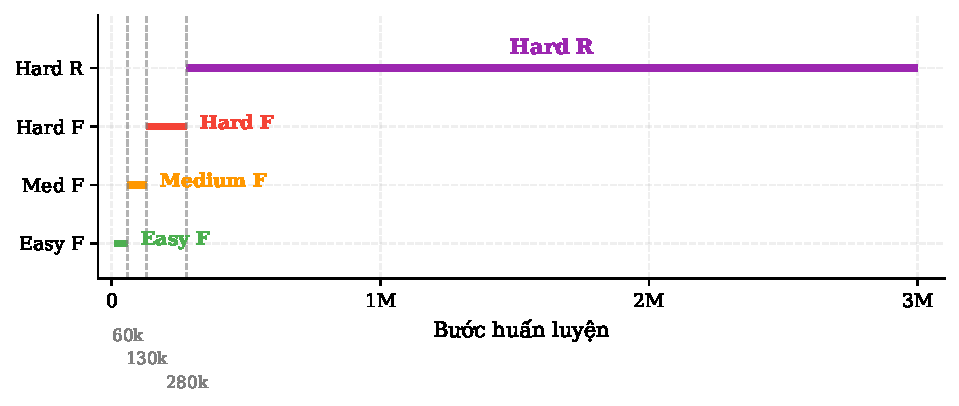
\includegraphics[width=0.85\textwidth]{figures/training/fig410_run54_four_tier.pdf}
    \caption{CL 4 bậc của run54: vị trí sinh cố định trước, vị trí sinh ngẫu nhiên sau}
    \label{fig:run54_four_tier}
\end{figure}

Vị trí sinh cố định giúp giảm phương sai ở giai đoạn đầu, nhưng khi chuyển sang mức Khó ngẫu nhiên thì tác nhân vẫn phải xử lý cùng nhóm bản đồ khó. Vì vậy, run54 chỉ cải thiện nhẹ ở hành vi chiến đấu và không làm thay đổi xu hướng tổng quát: CL là yếu tố chính trong nhóm thí nghiệm này, còn chuyển từ vị trí sinh cố định sang ngẫu nhiên là một biến thể thiết kế môi trường có tác động nhỏ hơn so với chính CL.

\subsection{Hàm thưởng v2 và thay đổi thang đo}
\label{sec:reward_v2_results}

Gắn với MT1, run55 kiểm tra liệu việc tăng trọng số phần thưởng kết quả có làm hành vi chiến đấu quyết đoán hơn hay không. Run55 thay đổi cấu trúc hàm thưởng: tăng mạnh phần thưởng tiêu diệt/dọn phòng/sát thương/tấn công đúng hướng, giảm phần thưởng tiếp cận và phạt mạnh hơn hành vi đứng gần địch không hành động. Run55 được huấn luyện đến 3.00M bước. Phần thưởng tail-50 đạt 9.600 và trung bình trên nhóm Khó đạt 9.337, nhưng không thể so sánh trực tiếp với run46 vì thang thưởng đã thay đổi.

Chỉ số đáng chú ý hơn là giá trị cực đại của tỷ lệ dọn phòng đạt 0.80, cao hơn mức 0.615 của run46. Khi nhấn mạnh kết quả, hàm thưởng v2 đẩy tác nhân tấn công quyết đoán hơn. Tuy nhiên entropy tail vẫn quanh 4.408 -- hàm thưởng v2 chưa giúp tác nhân thoát khỏi vùng bão hòa entropy.

Do đó, run55 được tách khỏi nhóm so sánh dùng hàm thưởng v1 khi diễn giải phần thưởng trung bình. Với hàm thưởng v2, các chỉ số phù hợp hơn để diễn giải là tỷ lệ dọn phòng, số kẻ địch tiêu diệt, sát thương gây ra, sát thương nhận vào, tỷ lệ sống sót hoặc các chỉ số đã chuẩn hóa theo cùng thang đo. Cách tách này tránh hiểu nhầm rằng giá trị phần thưởng 9.337 của run55 có thể so sánh trực tiếp với 3.843 của run46.

\begin{figure}[H]
    \centering
    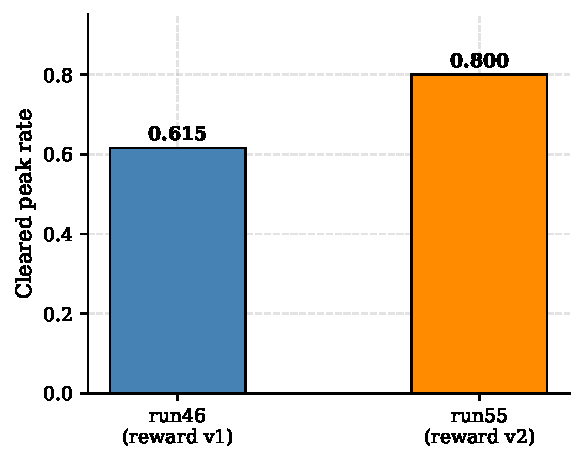
\includegraphics[width=0.55\textwidth]{figures/training/fig411_reward_v2_clear_peak.pdf}
    \caption{Ảnh hưởng của hàm thưởng v2 đến tỷ lệ dọn phòng cực đại}
    \label{fig:reward_v2_clear_peak}
\end{figure}

\section{Bão hòa entropy và nút thắt quan sát}
\label{sec:entropy_group}

Sau khi so sánh các kỹ thuật huấn luyện, một hiện tượng xuyên suốt hầu hết cấu hình là entropy chính sách bão hòa quanh 4.40 nat và không giảm dù đã áp dụng ICM, RND, LSTM, CL hoặc thiết kế lại phần thưởng. Nhóm thí nghiệm này phân tích nguyên nhân và kiểm tra giả thuyết rằng nút thắt chính nằm ở biểu diễn quan sát.

\subsection{Hiện tượng bão hòa entropy}
\label{sec:entropy_plateau_results}

Sau khi so sánh các kỹ thuật huấn luyện, một hiện tượng lặp lại trên hầu hết cấu hình là entropy của chính sách gần như không giảm khỏi vùng 4.40 nat. Với entropy cực đại lý thuyết $H_{\max}\approx 5.49$ nat ở phương trình~\ref{eq:max_entropy}, mức 4.40 tương đương khoảng 80\% của cực đại. Do cơ chế lọc hành động hợp lệ có thể làm cực đại thực tế thấp hơn, không nên diễn giải đây là chính sách hoàn toàn ngẫu nhiên; tuy vậy, chính sách vẫn giữ mức ngẫu nhiên cao. Hiện tượng này gắn trực tiếp với MT3 và mở đường cho phân tích nút thắt quan sát ở MT4.

\begin{figure}[H]
    \centering
    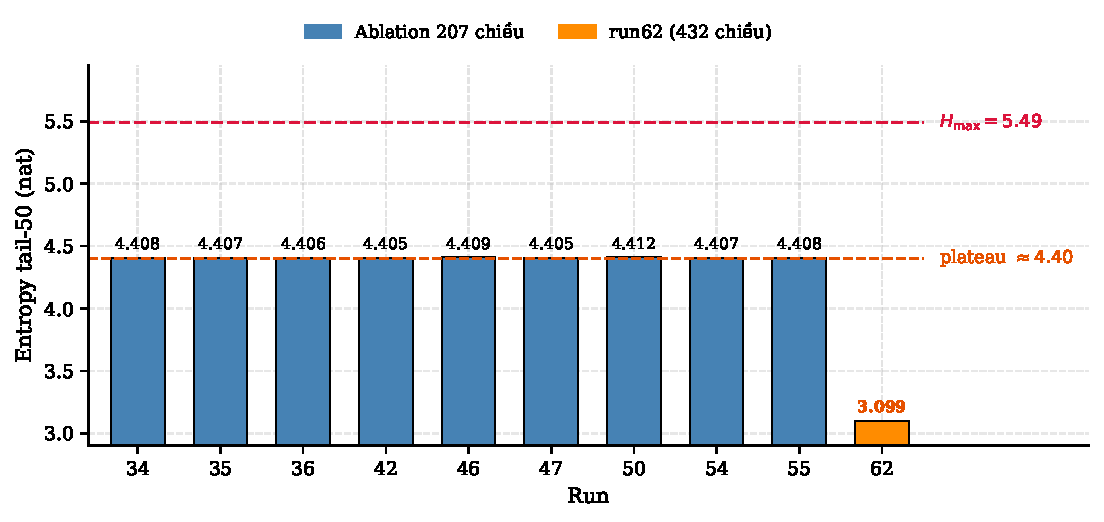
\includegraphics[width=0.95\textwidth]{figures/training/fig412_entropy_plateau.pdf}
    \caption{Entropy tail-50 của các lần chạy chính. Cấu hình run62 (40.82M bước, kết hợp lưới không gian cục bộ, CL 4 bậc và ICM) thoát khỏi vùng bão hòa 4.40 nat.}
    \label{fig:entropy_plateau}
\end{figure}

Trong các thí nghiệm cô lập biến chính giữ nguyên quan sát 207 chiều, vùng bão hòa này không được giải quyết bởi ICM, RND, LSTM, CL, giảm phương sai vị trí sinh hay thiết kế lại phần thưởng. Khi run62 kết hợp lưới không gian cục bộ với CL 4 bậc, ICM và được huấn luyện đến 40.82M bước, entropy giảm bền vững xuống 3.05 nat và duy trì ở mức này. Diễn giải thận trọng là: vùng bão hòa không phải giới hạn cứng của PPO hay không gian hành động hiện tại. Tuy nhiên, do chưa có cấu hình 207 chiều được huấn luyện tới 40M bước, khóa luận chưa thể loại trừ hoàn toàn khả năng vùng bão hòa ở các run trước một phần đến từ quy mô huấn luyện chưa đủ.

\subsection{Tác động của tín hiệu dẫn đường}
\label{sec:run59_path_informed}

Nhóm thí nghiệm mở rộng này trả lời Q3, tức kiểm tra vai trò của biểu diễn quan sát và tín hiệu điều hướng đối với khả năng dọn phòng. Sau các thí nghiệm cô lập biến chính, đề tài thực hiện thêm run59 để kiểm tra giả thuyết rằng giới hạn lớn nằm ở biểu diễn quan sát chứ không chỉ ở thuật toán học. Ở các cấu hình 207 chiều trước đó, tác nhân chỉ nhận các đặc trưng cục bộ về bản thân, kẻ địch, đạn và tường xung quanh; do đó, khi bản đồ có nhiều vật cản, chính sách phải tự suy ra hướng tiếp cận mục tiêu từ tín hiệu gián tiếp và phần thưởng bị trì hoãn. Run59 bổ sung ba chiều tín hiệu BFS vào CombatAgent: hướng bước kế tiếp trên đường đi ngắn nhất, khoảng cách đường đi ngắn nhất đã chuẩn hóa tới kẻ địch còn sống gần nhất và thông tin hỗ trợ tiếp cận mục tiêu, làm vector quan sát tăng từ 207 lên 210 chiều. Các tín hiệu này không trực tiếp quyết định hành động thay cho tác nhân, nhưng làm rõ cấu trúc đường đi trong bản đồ có tường và giảm gánh nặng suy luận điều hướng từ quan sát thô. Vì vậy, run59 không được xem là cấu hình RL thuần hay thí nghiệm cô lập biến ngang hàng với các lần chạy chính. Thay vào đó, run này được dùng như thí nghiệm mở rộng nhằm ước lượng hiệu năng khi nút thắt điều hướng được hỗ trợ, trong khi tác nhân vẫn phải tự học cách phối hợp di chuyển, ngắm, tấn công, lướt và lựa chọn thời điểm giao tranh phù hợp.

Về mặt phương pháp, run59 là một phép can thiệp có chủ đích vào kênh quan sát. Không gian hành động, mục tiêu dọn phòng và các yêu cầu chiến đấu cốt lõi vẫn giữ nguyên, nhưng tác nhân được cung cấp thêm một gợi ý có cấu trúc về đường đi. Vì vậy, khi đọc kết quả của run này, cần quan sát đồng thời ba nhóm chỉ số: chỉ số kết quả như phần thưởng, số kẻ địch bị tiêu diệt và tỷ lệ dọn phòng; chỉ số về chính sách như entropy để xem tác nhân có bớt dao động trong lựa chọn hành động hay không; và chỉ số nhiễu môi trường như số lần kẻ địch thoát kẹt để đánh giá mức độ ổn định của tập mẫu huấn luyện. Cách đọc này giúp tránh diễn giải run59 như một chiến thắng tuyệt đối của thuật toán, mà xem nó như bằng chứng về mức độ ảnh hưởng của thông tin điều hướng đối với toàn bộ vòng lặp học.

\begin{table}[H]
    \centering
    \small
    \caption{Kết quả cấu hình run59 với tín hiệu dẫn đường}
    \label{tab:run59_bfs_assisted}
    \begin{tabular}{|p{4.1cm}|p{3.7cm}|p{6.4cm}|}
        \hline
        \textbf{Chỉ số} & \textbf{Giá trị cuối quá trình huấn luyện} & \textbf{Diễn giải} \\
        \hline
        Phần thưởng tích lũy & 14.09 cuối quá trình huấn luyện; tail ở vùng cuối khoảng 14.77 & Cao hơn rõ so với các lần chạy chính, nhưng không so sánh trực tiếp vì quan sát và định hình phần thưởng đã thay đổi. \\
        \hline
        Tỷ lệ dọn phòng & 0.727 cuối quá trình huấn luyện; tail ở vùng cuối khoảng 0.846 & Tác nhân dọn phòng ổn định hơn khi được cung cấp tín hiệu đường đi. \\
        \hline
        Số kẻ địch bị tiêu diệt/lượt & 1.55 cuối quá trình huấn luyện; tail ở vùng cuối khoảng 1.78 & Số kẻ địch bị tiêu diệt tăng, cho thấy khả năng điều hướng là một nút thắt thực tế của bài toán. \\
        \hline
        Entropy chính sách & Giảm từ khoảng 4.15 xuống 3.59; tail ở vùng cuối khoảng 3.62 & Chính sách trở nên quyết đoán hơn so với các lần chạy bị bão hòa quanh 4.40 nat. \\
        \hline
        Phần thưởng nội tại (ICM) & Khoảng 0.005 ở cuối quá trình huấn luyện & ICM không còn chi phối hành vi ở cuối quá trình huấn luyện. \\
        \hline
        Số lần kẻ địch thoát kẹt & Tail ở vùng cuối khoảng 3.07 mỗi lượt chơi & Môi trường vẫn còn nhiễu do kẻ địch bị kẹt hoặc cần phục hồi, nên kết quả cần được diễn giải cùng hạn chế về thời gian chạy. \\
        \hline
    \end{tabular}
\end{table}

Bảng~\ref{tab:run59_bfs_assisted} cho thấy khi bổ sung tín hiệu dẫn đường, các chỉ số hành vi tăng mạnh: tỷ lệ dọn phòng đạt trên 0.8 ở vùng cuối, số kẻ địch bị tiêu diệt trung bình vượt 1.7 và entropy giảm sâu hơn so với vùng bão hòa của các lần chạy 207 chiều. Đây là mức cải thiện lớn nhất trong quá trình thử nghiệm, nhưng cần diễn giải như mốc tham chiếu có hỗ trợ điều hướng. Kết quả cho thấy nút thắt chính không chỉ nằm ở PPO hay cơ chế khám phá, mà còn ở biểu diễn không gian của quan sát. Các hướng tiếp theo nên tập trung vào lưới không gian cục bộ, đặc trưng đồ thị/đường đi học được, học bắt chước cho điều hướng, hoặc thiết kế lại bản đồ/kẻ địch để giảm nhiễu từ các tình huống kẹt.

Run59 mang lại bước cải thiện lớn nhất về hiệu năng thực nghiệm, nhưng bản chất của cải thiện đến từ thay đổi biểu diễn quan sát chứ không chỉ từ thuật toán học. Kết quả không chứng minh tác nhân đã tự học tìm đường hoàn toàn; nó chỉ cho thấy khi được cung cấp tín hiệu dẫn đường phù hợp hơn, chính sách có thể học hành vi chiến đấu và tiếp cận mục tiêu ổn định hơn.

\subsection{Lưới không gian cục bộ trong huấn luyện trực tiếp}
\label{sec:run62_local_grid}

Sau khi run59 cho thấy tín hiệu điều hướng tạo cải thiện rõ rệt, run62 được thiết kế như một cấu hình mở rộng để kiểm tra liệu tác nhân có thể tiến gần mức hiệu năng đó mà không nhận trực tiếp hướng đi tối ưu hay không -- mục tiêu là để tác nhân tự khai thác bố cục không gian cục bộ thay vì dựa vào BFS. Cấu hình này thay quan sát 207 chiều bằng lưới cục bộ $15 \times 15$ (432 chiều), kết hợp CL 4 bậc, ICM hệ số 0.001 và \textbf{aggressive\_seek} để kẻ địch truy đuổi chủ động hơn, huấn luyện trên 8 môi trường song song qua hai phiên chạy tổng cộng \textbf{40.82M bước}. Vì thay đổi đồng thời quan sát, CL, ICM, siêu tham số và thời lượng huấn luyện, run62 được xem là bằng chứng thăm dò của một cấu hình kết hợp, không phải thí nghiệm đơn biến cho riêng lưới không gian cục bộ.

\begin{figure}[H]
    \centering
    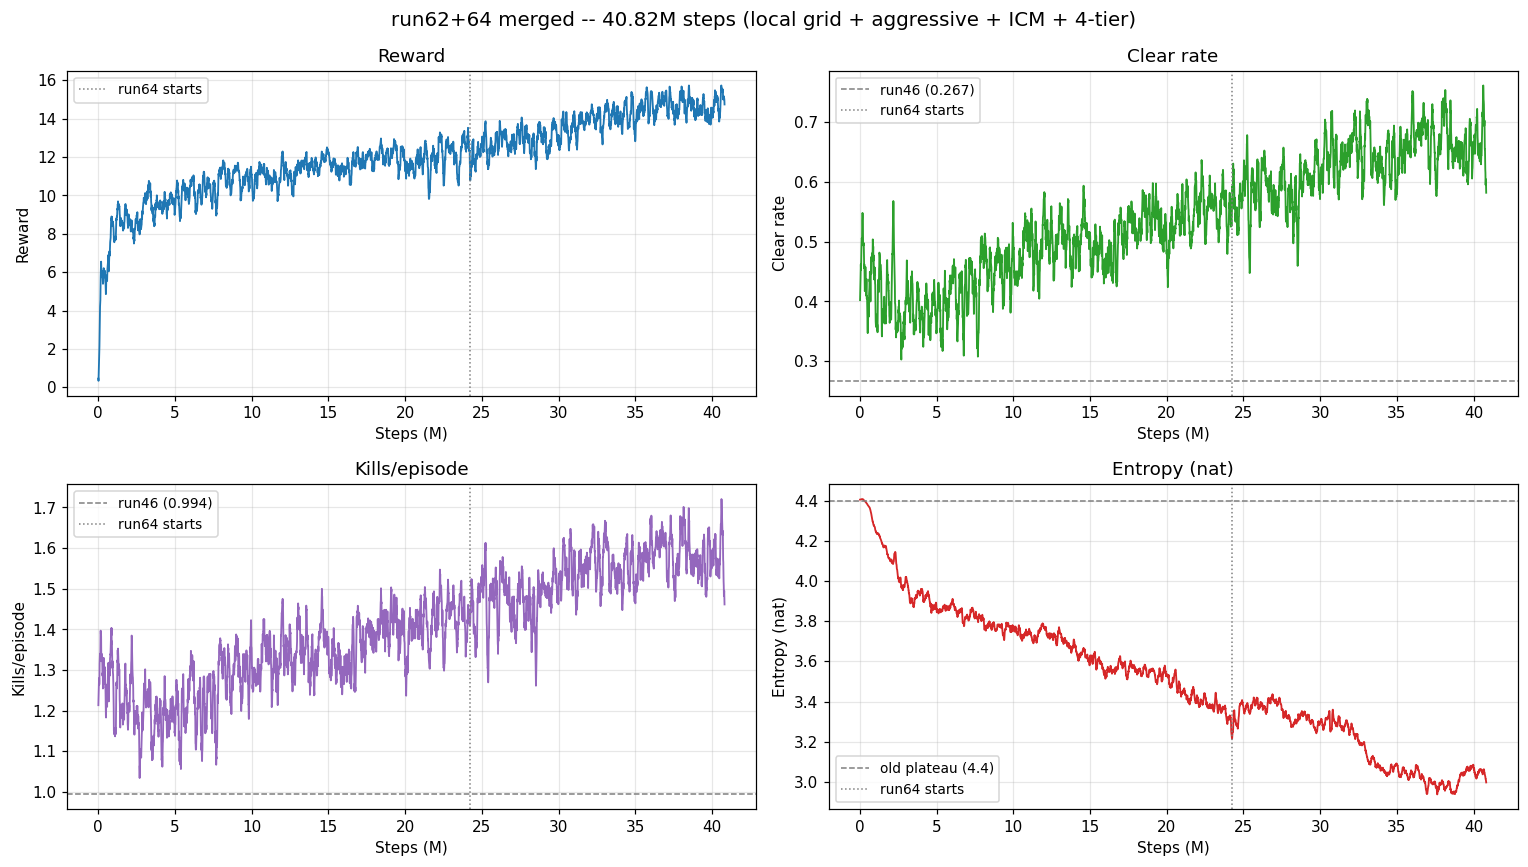
\includegraphics[width=1\textwidth]{figures/training/run62_merged_overview.png}
    \caption{Tổng quan quá trình huấn luyện 40.82M bước: phần thưởng, tỷ lệ dọn phòng, số kẻ địch tiêu diệt và entropy. Đường kẻ dọc đánh dấu điểm bắt đầu phiên chạy thứ hai (24.25M bước).}
    \label{fig:run62_merged_overview}
\end{figure}

Sau 40.82M bước huấn luyện, phần thưởng tail-50 đạt 14.913 (giá trị cực đại 19.695), số kẻ địch tiêu diệt tail-50 đạt 1.582 -- gần chạm giới hạn trên 2 kẻ địch mỗi phòng, tỷ lệ dọn phòng tail-50 đạt 0.666 và tỷ lệ lướt hữu ích đạt 0.439. Tỷ lệ dọn phòng 0.666 nằm giữa run46 CL cơ sở (0.267) và run59 có hỗ trợ BFS (0.846), thu hẹp khoảng 69\% khoảng cách tới run59 dù không được cung cấp trực tiếp hướng đi tối ưu mà chỉ dùng lưới không gian cục bộ. Kết quả này cho thấy cấu hình mở rộng có tiềm năng tiệm cận cấu hình có hỗ trợ BFS, nhưng chưa đủ để quy riêng cải thiện cho lưới không gian cục bộ.

Kết quả đáng chú ý hơn nằm ở diễn biến entropy: chỉ số này giảm bền vững từ vùng bão hòa 4.40 nat của các thí nghiệm cô lập biến 1--3M bước xuống còn 3.048 tail-50, tức thấp hơn 1.35 nat so với mức cũ, với quỹ đạo giảm đơn điệu thay vì dao động quanh một điểm cố định. Đây là lần đầu tiên chính sách thoát khỏi vùng bão hòa entropy, cho thấy 4.40 nat không phải giới hạn cứng mà là điểm bão hòa phụ thuộc điều kiện huấn luyện; tuy nhiên vì run62 thay đổi nhiều yếu tố đồng thời, chưa thể xác định lưới không gian cục bộ là yếu tố duy nhất quyết định kết quả này.

\begin{figure}[H]
    \centering
    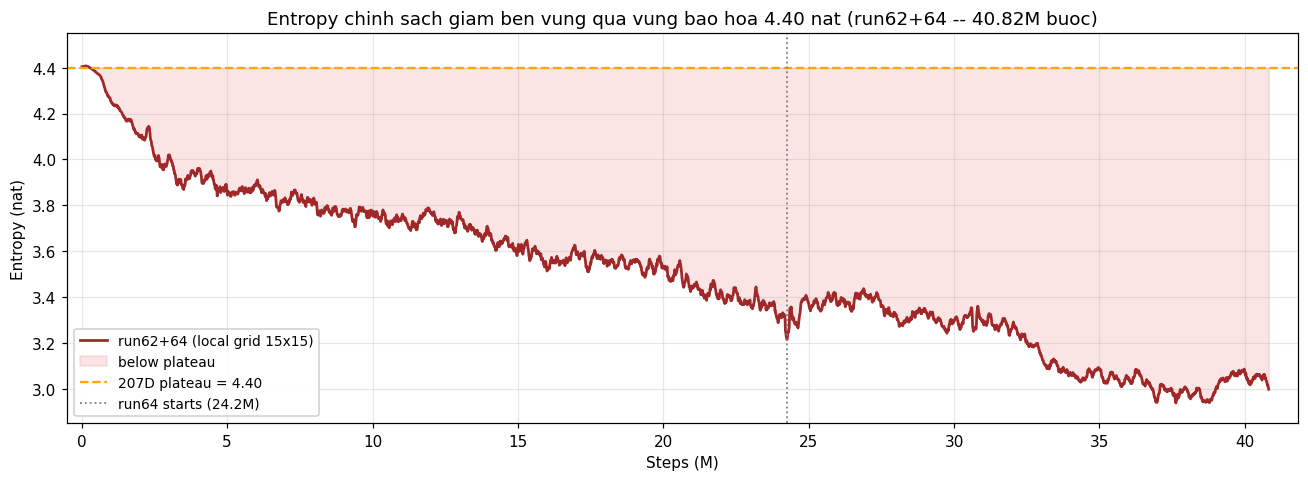
\includegraphics[width=0.98\textwidth]{figures/training/run62_merged_entropy.png}
    \caption{Entropy chính sách giảm xuống dưới vùng bão hòa 4.40 nat và duy trì bền vững. Vùng tô màu biểu thị khoảng entropy nằm dưới mức cũ.}
    \label{fig:run62_merged_entropy}
\end{figure}

Khác với run59, run62 không nhận trực tiếp hướng đi tối ưu mà chỉ dùng lưới không gian cục bộ. Dù tỷ lệ dọn phòng 0.666 vẫn thấp hơn cấu hình có tín hiệu BFS, kết quả này cho thấy quan sát mô tả tốt hơn bố cục quanh tác nhân có thể giúp chính sách học hành vi tiếp cận, né kẹt và duy trì giao tranh ổn định hơn so với quan sát vector 207 chiều ban đầu.


\section{Tổng hợp kết quả}
\label{sec:results_summary}

\begin{table}[H]
    \centering
    \footnotesize
    \setlength{\tabcolsep}{3.5pt}
    \renewcommand{\arraystretch}{1.22}
    \caption{Tổng hợp các cấu hình thí nghiệm chính}
    \label{tab:master_ablation}
    \begin{tabular}{|>{\raggedright\arraybackslash}p{1.15cm}|>{\raggedright\arraybackslash}p{2.65cm}|>{\centering\arraybackslash}p{1.05cm}|>{\centering\arraybackslash}p{1.95cm}|>{\centering\arraybackslash}p{1.35cm}|>{\raggedright\arraybackslash}p{6cm}|}
        \hline
        \textbf{Run} & \textbf{Thiết lập} & \textbf{Bước} & \textbf{Reward} & \textbf{Kills} & \textbf{Kết luận} \\
        \hline
        run34 & PPO cơ sở & 1.0M & 2.073 & 0.721 & Mốc so sánh; học được chiến đấu cơ bản nhưng đạt trần ở mức thấp. \\
        \hline
        run35 & PPO + ICM & 1.0M & 2.416 & 0.752 & Cải thiện nhỏ; mất mát của mô hình ngược chưa thấp hơn rõ vùng entropy chính sách. \\
        \hline
        run36 & PPO + RND & 1.0M & 2.487 & 0.796 & Nhỉnh hơn ICM nhẹ, nhưng chưa tạo cải thiện đáng chú ý. \\
        \hline
        run42 & PPO + LSTM & 1.0M & 2.411 & 0.769 & Học chậm nhưng tăng dần; lợi ích hạn chế. \\
        \hline
        run46 & PPO + CL & 3.0M & 3.843 & 0.994 & Cải thiện nổi bật, kill/episode và tỷ lệ dọn phòng đều tăng rõ. \\
        \hline
        run47 & CL + LSTM & 3.0M & 3.765 & 0.921 & Chưa cho thấy tác dụng bổ trợ rõ với CL. \\
        \hline
        run50 & CL + ICM & 3.0M & 4.369 & 1.016 & Bổ trợ nhẹ với CL; mất mát của mô hình ngược chưa thấp hơn rõ vùng entropy chính sách. \\
        \hline
        run54 & 4 bậc, cố định--ngẫu nhiên & 3.0M & 3.925 & 0.945 & Tương đương run46; biến thể vị trí sinh cố định--ngẫu nhiên chỉ cải thiện nhẹ. \\
        \hline
        run55 & CL + hàm thưởng v2 & 3.0M & 9.337 & 1.014 & Giá trị cực đại của tỷ lệ dọn phòng cao hơn; thang thưởng khác nên không so sánh trực tiếp giá trị trung bình. \\
        \hline
        run62 & Lưới cục bộ + {aggressive\_seek} + ICM + 4 bậc & 40.82M & 14.913 & 1.582 & Entropy 3.05 -- thoát khỏi vùng bão hòa cũ; tỷ lệ dọn phòng 0.666; tiệm cận cấu hình có hỗ trợ BFS dù không dùng trực tiếp tín hiệu BFS. \\
        \hline
    \end{tabular}
\end{table}

Bảng~\ref{tab:master_ablation} cho thấy PPO cơ sở học được hành vi chiến đấu cơ bản nhưng còn giới hạn; ICM, RND và LSTM chỉ cải thiện nhẹ khi chạy độc lập. CL là yếu tố nổi bật nhất, và khi kết hợp thêm ICM ở run50, phần thưởng tiếp tục tăng nhưng mất mát của mô hình ngược vẫn gần vùng entropy chính sách. Với run62, entropy giảm xuống 3.048 nat và tỷ lệ dọn phòng đạt 0.666, cho thấy vùng bão hòa 4.40 nat có thể vượt qua; tuy nhiên vì cấu hình này thay đổi nhiều yếu tố đồng thời nên kết quả chỉ mang tính thăm dò. Các số liệu này là cơ sở định lượng chính cho phần kết luận ở Chương~5.



\begin{figure}[H]
    \centering
    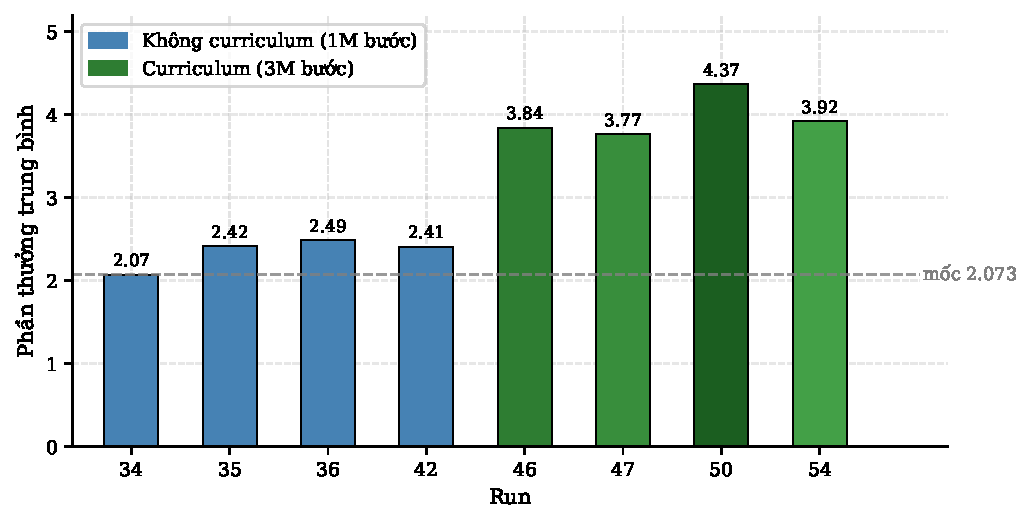
\includegraphics[width=0.9\textwidth]{figures/training/fig413_reward_comparison.pdf}
    \caption{So sánh phần thưởng trung bình giữa các cấu hình dùng hàm thưởng v1.}
    \label{fig:reward_comparison_all}
\end{figure}

\begin{figure}[H]
    \centering
    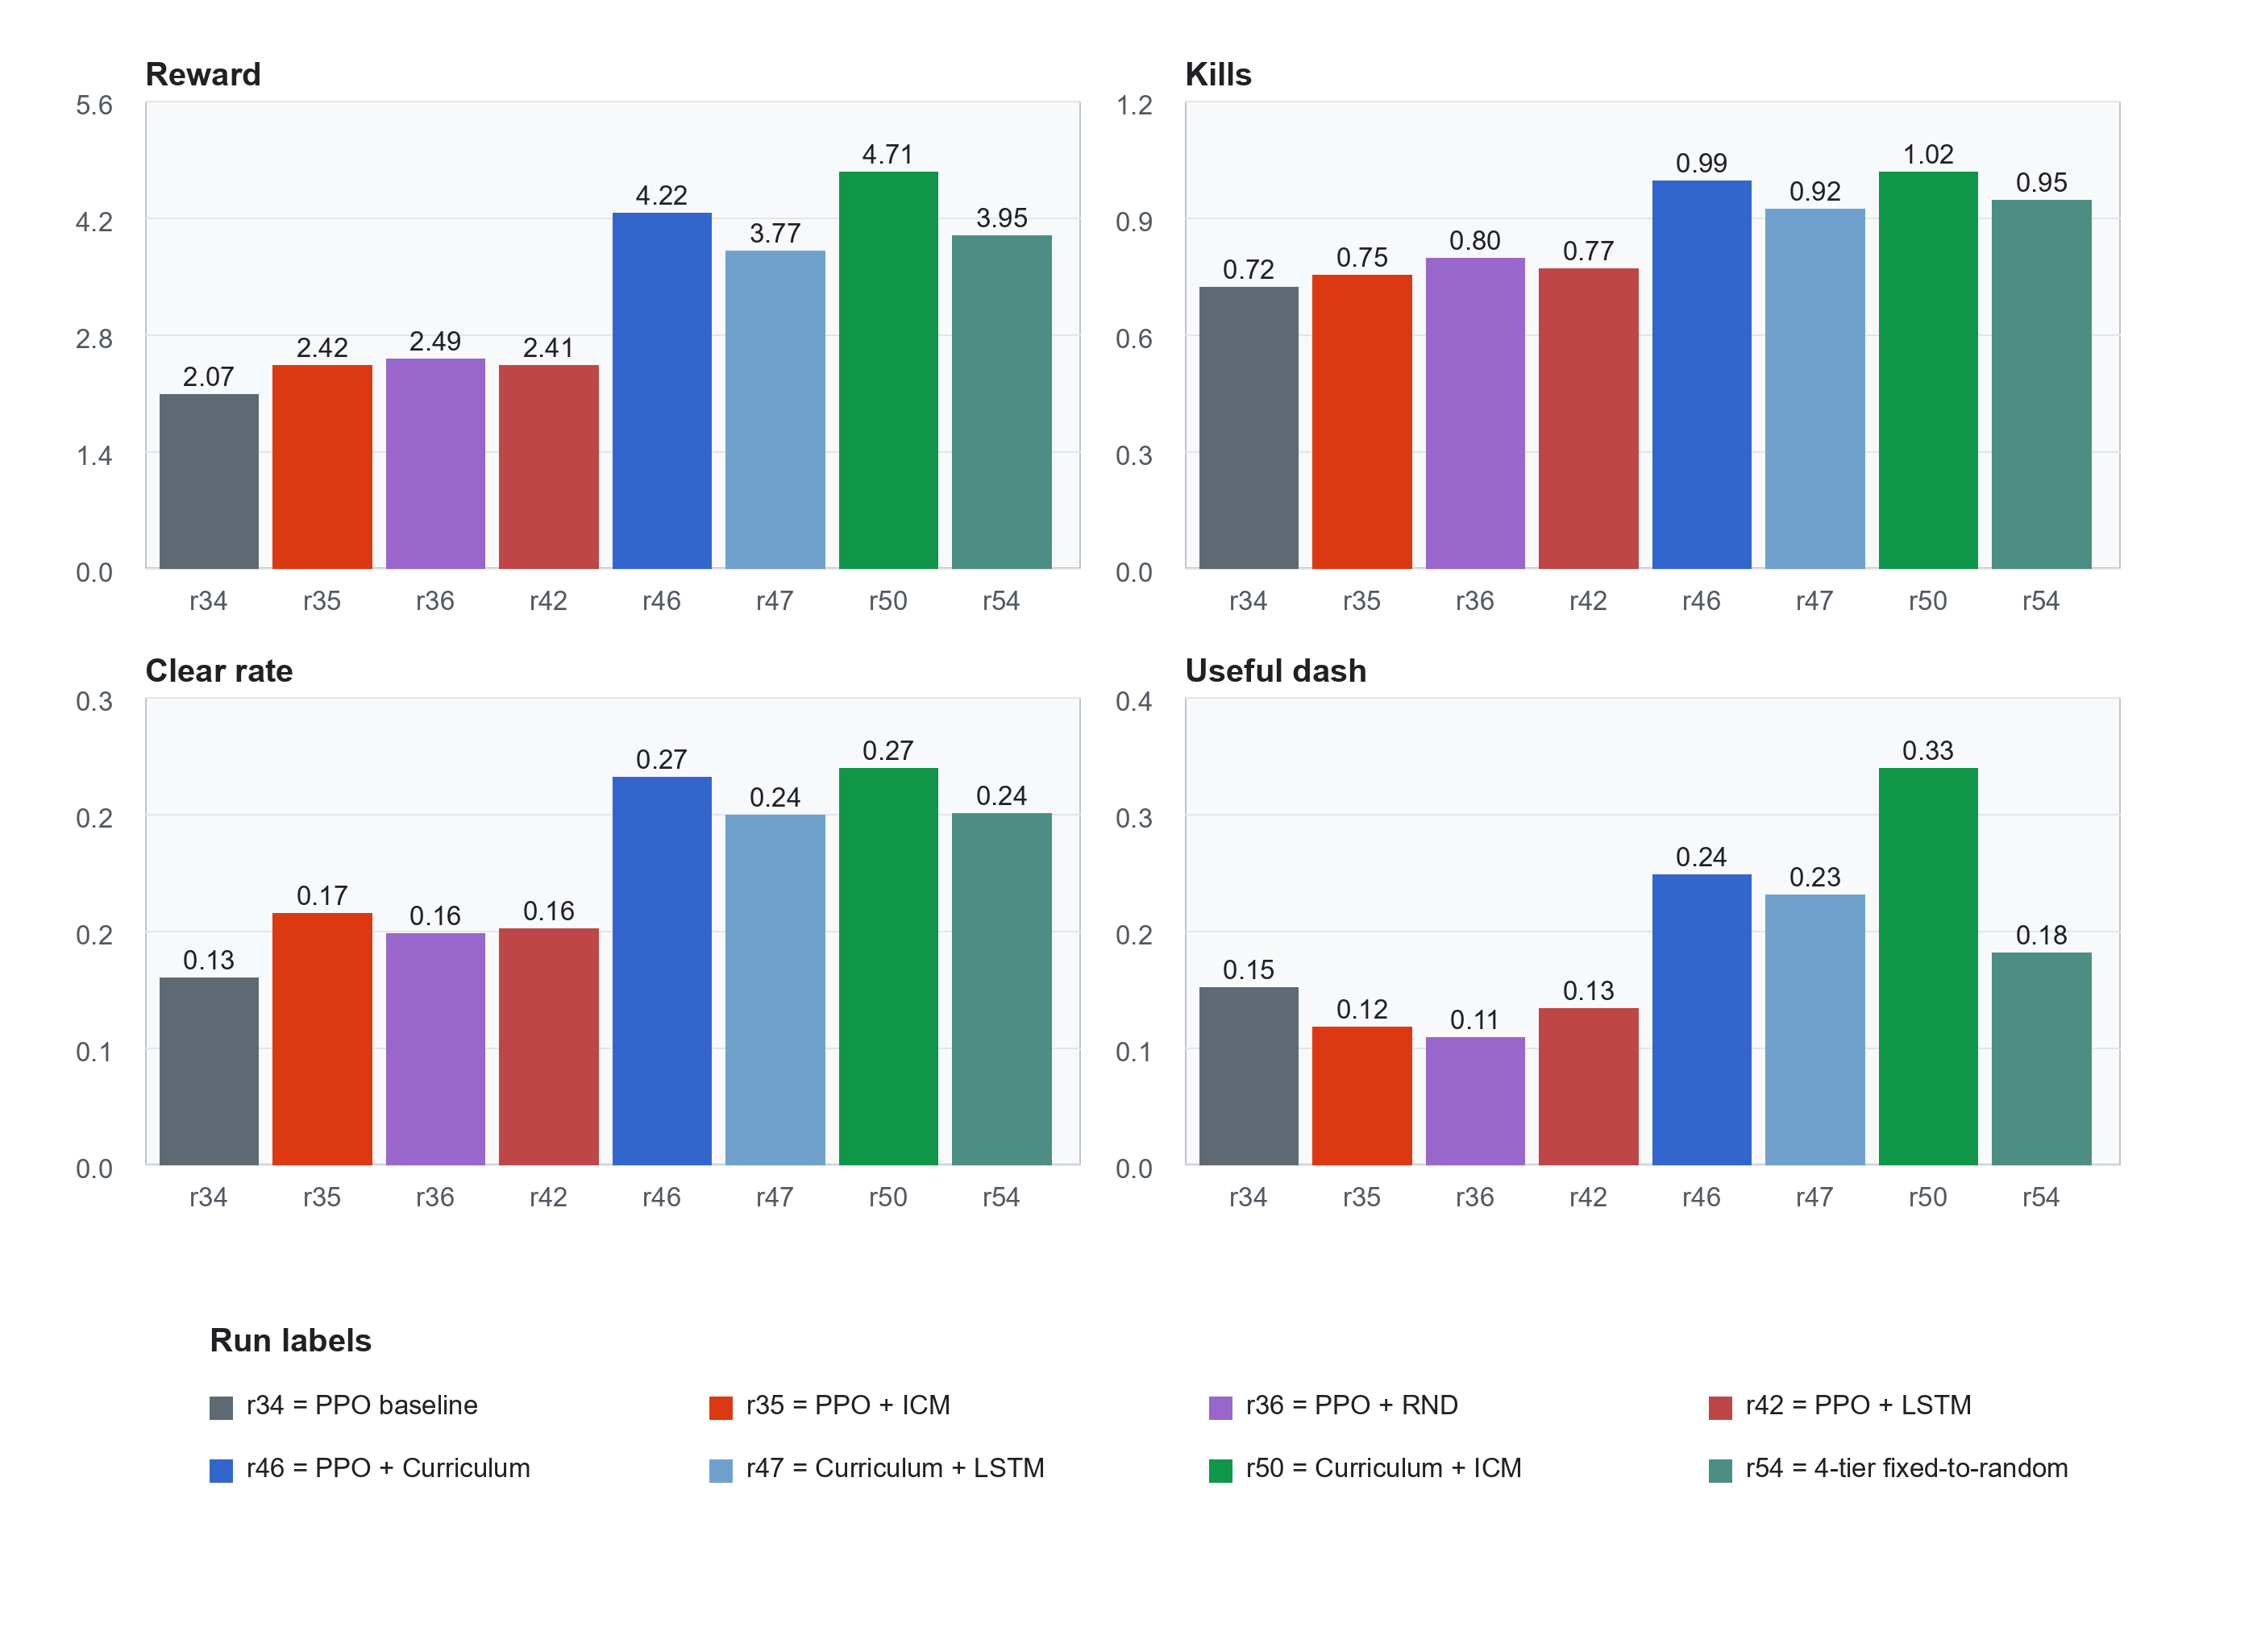
\includegraphics[width=0.98\textwidth]{figures/training/final_metrics_comparison.png}
    \caption{So sánh các chỉ số hành vi ở cuối quá trình huấn luyện. Hình bổ sung cho Bảng~\ref{tab:run_metrics_main}: CL không chỉ tăng phần thưởng mà còn cải thiện số kẻ địch bị tiêu diệt, tỷ lệ dọn phòng và tỷ lệ lướt hữu ích.}
    \label{fig:final_metrics_comparison}
\end{figure}
